\cleardoublepage

\begin{frontmatter}
	\chapter{Análise Matricial de Estruturas}
\end{frontmatter}

\section{Métodos de Análise}

Existem dois grandes métodos em análise matricial de estruturas, que são, o \underline{Método da Flexibilidade} (baseado em forças ou ações) e o \underline{Método da Rigidez} (baseado em deslocamentos), que se aplicam a qualquer tipo de estrutura, e das quais se derivam outros métodos de análise estrutural. As características gerais desses métodos são mostradas a seguir.

\bigskip

\noindent \textbf{Método das Forças (M.F.):}
\begin{enumerate}
	\item
	      As equações para um sistema estrutural são estabelecidas em termos de \underline{ações} de extremidades de membros. Tem-se, para problemas hiperestáticos, equações de compatibilidade de deslocamento além das equações de equilíbrio pertinentes.
	\item
	      Para um mesmo sistema estrutural há diversos sistemas principais de análise (obtidos pelo rompimento do sistema original na direção das redundantes incógnitas).
	\item
	      Para a obtenção de respostas em termos de deslocamentos, faz-se necessário a utilização de outros métodos (por exemplo, Princípio dos Trabalhos Virtuais).
	\item
	      Por haver diversas possibilidades de sistemas principal, o método não é muito adequado para a implementação computacional.
	\item
	      Por descrever a resposta dos sistemas em termos de ações, o método das forças também não é apropriado para a realização de análises dinâmicas (em que há grandezas do tipo aceleração e velocidade, obtidas das funções de deslocamentos via diferenciações temporais).
\end{enumerate}

\bigskip

\noindent \textbf{Método dos Deslocamentos (M.D.):}
\begin{enumerate}
	\item
	      As equações para um sistema estrutural são estabelicidas em termos de \underline{deslocamentos} nodais. Na verdade, tem-se um conjunto de equações de equilíbrio nodal.
	\item
	      Definidos os nós estruturais e respectivos elementos, o estabelecimento do sistema de equações é direto (e único). O método é, portanto, muito adequado para a implementação computacional.
	\item
	      De posse dos deslocamentos nodais, o cálculo das ações de extremidade do membro é também direto.
	\item
	      O método é também apropriado para a realização de análises dinâmicas.
\end{enumerate}

Conceitos importantes associados a esses métodos são o de \underline{indeterminação estática} e \underline{cinemática}, os quais se relacionam, respectivamente, ao \underline{M.F.} e ao \underline{M.D.}

A \underline{indeterminação estática} (i.e.) é o excesso de ações incógnitas em relação ao número de equações de equilíbrio disponíveis. Este conceito relaciona-se naturalmente com o M.F., que formula sistemas estruturais em termos de ações. Neste caso, o número de ações incógnitas excessivas ou redundantes define o grau de indeterminação estática da estrutura (grau de hiperestaticidade).

Já a \underline{indeterminação cinemática} (i.c.) associa-se ao número de deslocamentos nodais desconhecidos em
formulações do M.D., que por sua vez, exatamente, corresponde ao grau de indeterminação cinemática ou número de graus de liberdade do sistema estrutural.

\bigskip

\noindent Exemplos: Determinação do grau de indeterminação estática e cinemática de estruturas

\begin{figure}[!htbp]
	\begin{subfigure}[]{0.49\textwidth}
		\centering
		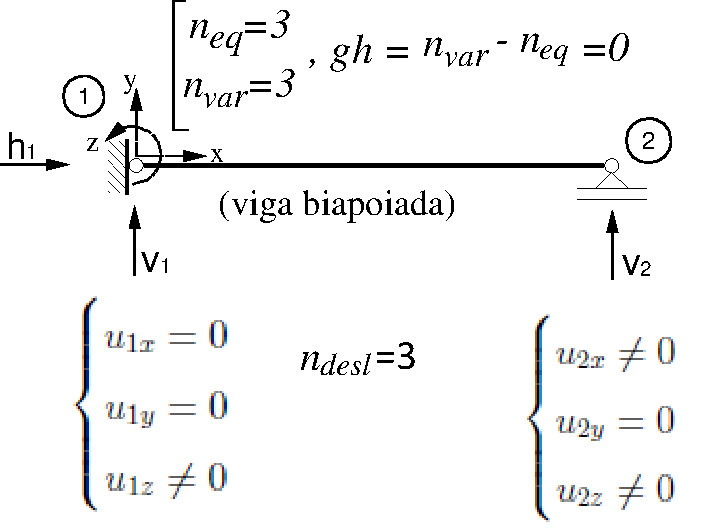
\includegraphics[scale=0.60]{img/ex-viga-iso}
	\end{subfigure}
	\begin{subfigure}[]{0.49\textwidth}
		\centering
		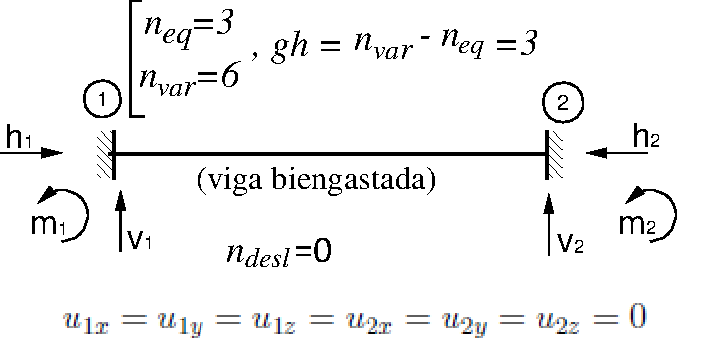
\includegraphics[scale=0.65]{img/ex-viga-hiper}
	\end{subfigure}
\end{figure}

\begin{figure}[!htbp]
	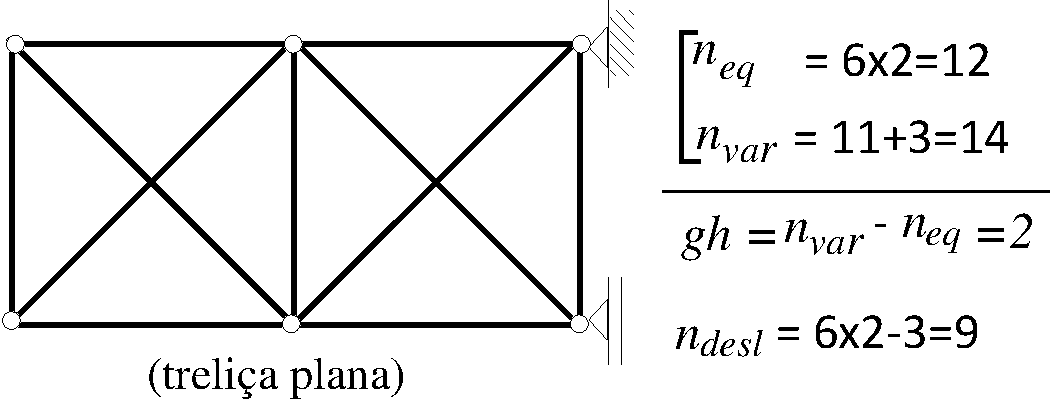
\includegraphics[scale=0.450]{img/ex-treliçaplana}
\end{figure}

\begin{figure}[!htbp]
	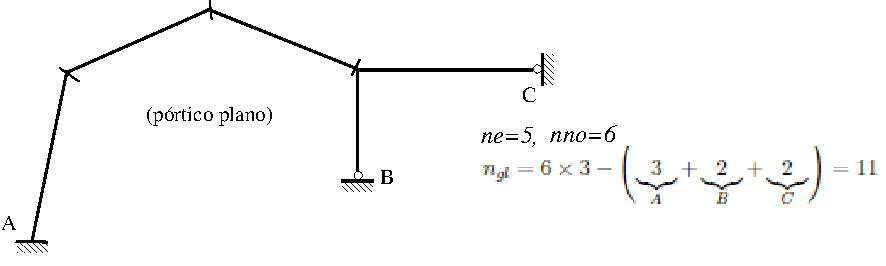
\includegraphics[scale=0.70]{img/port-plano1-ic}
\end{figure}

\begin{figure}[!htbp]
	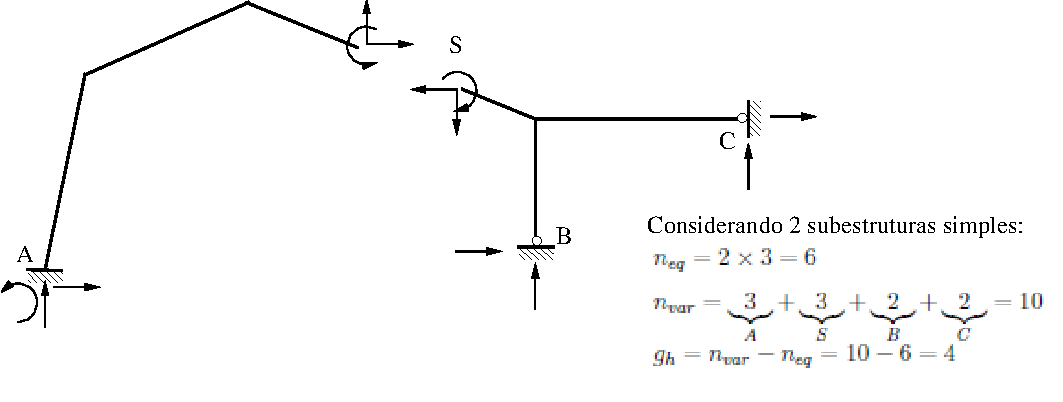
\includegraphics[scale=0.75]{img/port-plano1-ie}
\end{figure}

\begin{figure}[!htbp]
	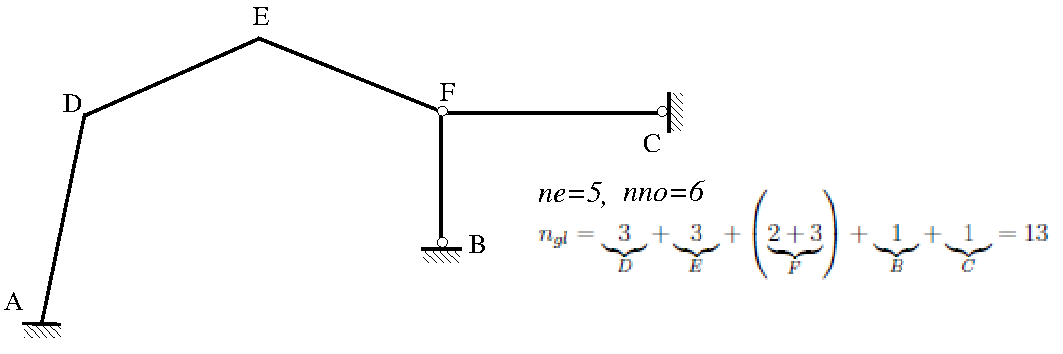
\includegraphics[scale=0.80]{img/port-plano2-ic}
\end{figure}

\begin{figure}[!htbp]
	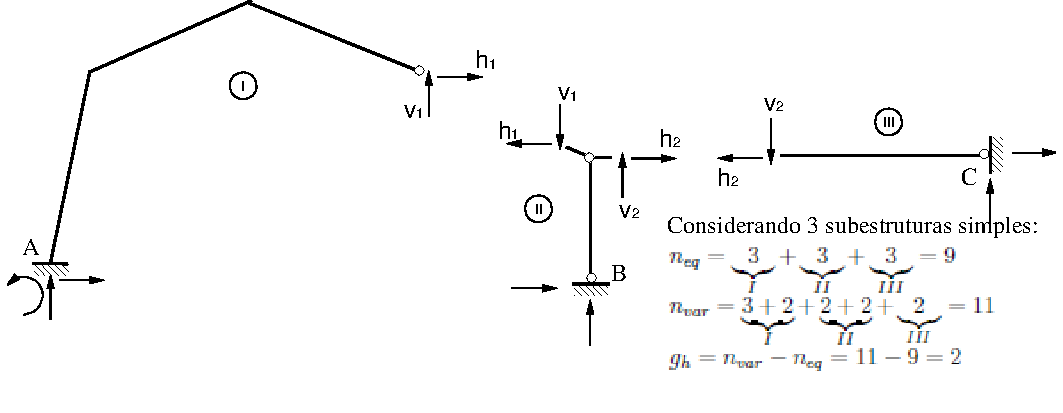
\includegraphics[scale=0.80]{img/port-plano2-ie}
\end{figure}

\begin{figure}[!htbp]
	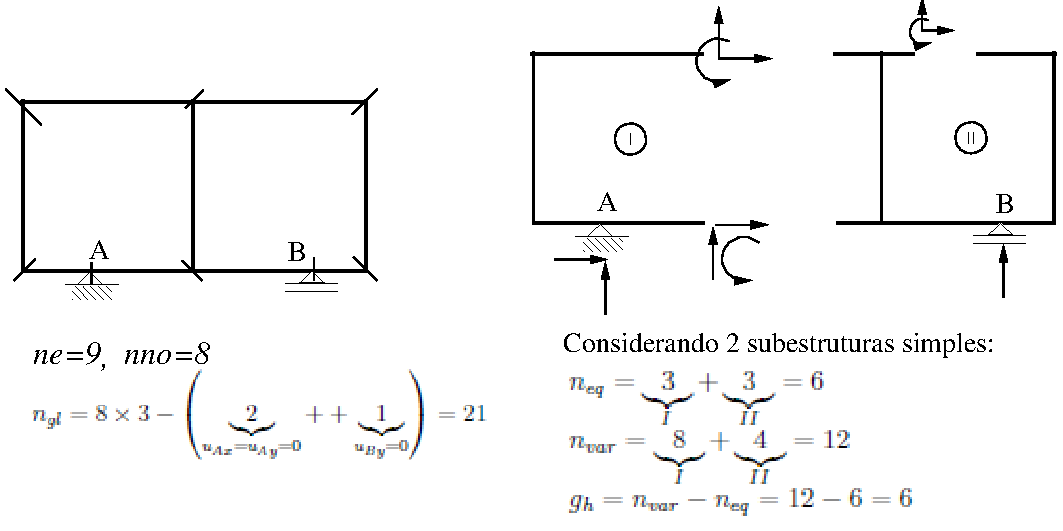
\includegraphics[scale=0.75]{img/port-plano3-fechado}
\end{figure}

\clearpage
\begin{figure}[!htbp]
	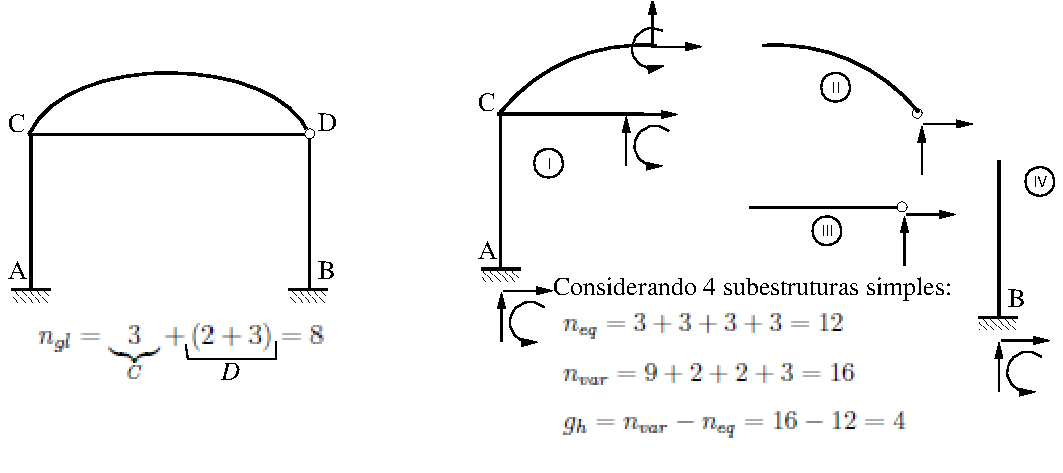
\includegraphics[scale=0.75]{img/port-plano4-fechado}
\end{figure}

\begin{figure}[!htbp]
	\centering
	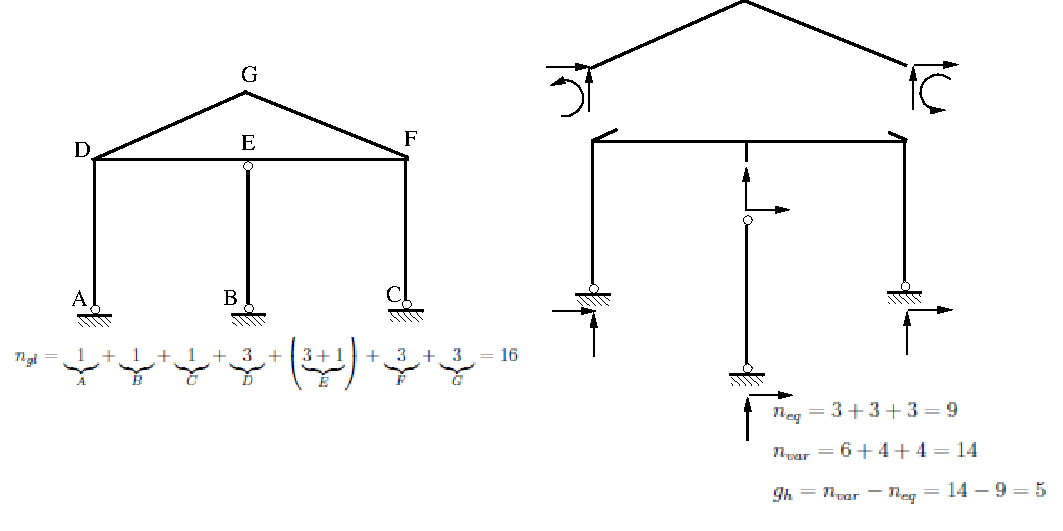
\includegraphics[scale=0.80]{img/port-plano5-fechado}
\end{figure}

\begin{figure}[!htbp]
	\centering
	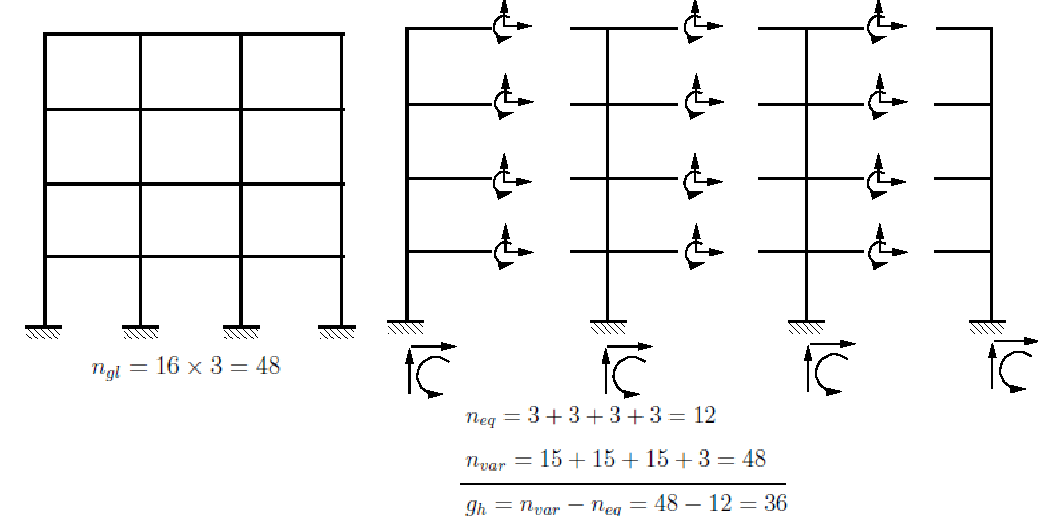
\includegraphics[scale=0.80]{img/port-plano6-fechado}
\end{figure}

\clearpage
\begin{figure}[!htbp]
	\centering
	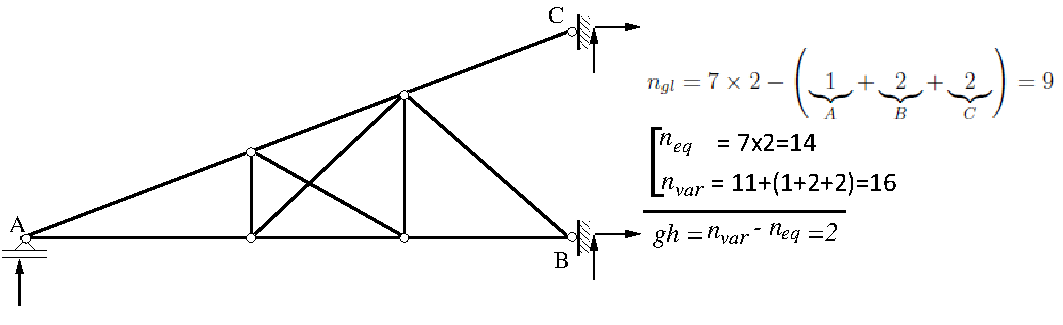
\includegraphics[scale=0.80]{img/treliçaplana2}
\end{figure}

\begin{figure}[!htbp]
	\centering
	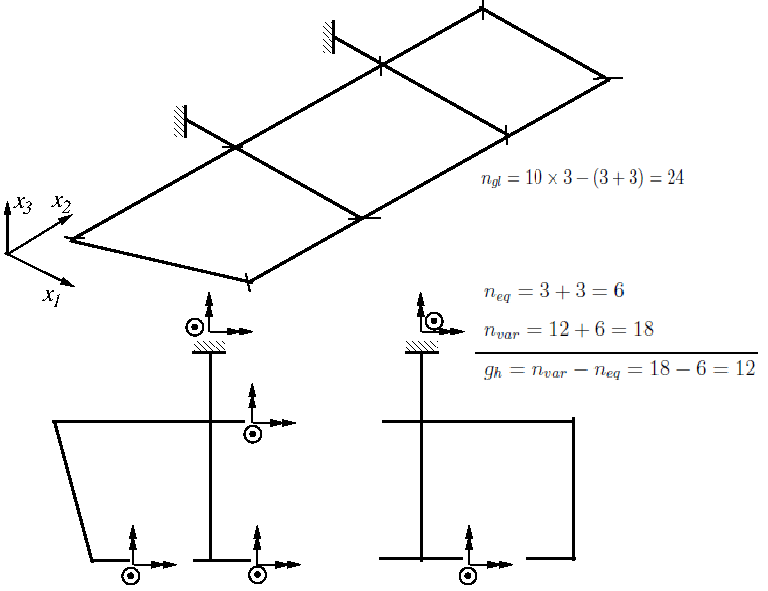
\includegraphics[scale=0.85]{img/grelha1}
\end{figure}

Observações:
\begin{enumerate}
	\item
	      O grau de indeterminação cinemática ($n_{gl}$) pode ser calculado em termos gerais pela expressão \[ n_{gl}\!=\!nno\times ndofn - n_{dr} \; ,\] sendo
	      \textit{nno} = nº de nós considerados no modelo, \textit{ndofn} = nº de graus de liberdade por nó, e $n_{dr}$ = nº de deslocamentos restringidos. Note que quanto maior o nº de nós do modelo, maior o grau de indeterminação cinemática.

	\item
	      O grau de indeterminação estática ($gh$) pode ser calculados por
	      \[g_{h}=\sum_{i}^{n_{sub}}\left [ n_{var}(i)-n_{eq}(i) \right ] \; ,\] onde
	      $n_{var}(i)$ = nº de ações incógnitas da i-ésima subestrutura e $n_{eq}(i)$ = nº de equações de equilíbrio da i-ésima subestrutura.
	      Há, naturalmente, diversas formas de partição da estrutura dada em subestruturas de interesse.

	\item
	      Note que o método das forças usualmente gera sistemas de equações com menos incógnitas do que aqueles que resultam da análise via método dos deslocamentos. Sendo assim, o método das forças é na verdade mais adequado para a resolução manual de estruturas (caso não se objetive calcular deslocamentos). Por outro lado, ressalta-se também que a implementação do método dos deslocamentos depende do método das forças, uma vez que grandezas básicas deste método, tais como coeficientes de rigidez e ações nodais equivalentes, são obtidos via método das forças.

	\item
	      Note que no método das forças, o número de ações incógnitas, $n_{var}$, e o número de equações, $n_{eq}$, para uma estrutura qualquer, dependerá do número de subestruturas ($n_{sub}$) adotadas na análise, que pode ser qualquer. O grau de hiperestaticidade, $g_h$, independerá, porém, de $n_{sub}$.
\end{enumerate}
